\chapter{Visualizing Scene Graphs} \label{chap:3}
Visualizing the richly structured geometric information contained in a generative scene graph model is vital for proper debugging and analysis of modeling and inference programs.
This chapter presents a series of visualization utilities for rendering distributions over scene graphs.
Thus this method serves as one of the main utilities used in data-exploration (neural detections are special case scene graphs with no edges), model development, and testing.

\section{Desiderata}
It is important to be able to clearly distinguish each part of a scene graph $(G, \Theta, Z)$; as will be seen later, incorrect behavior in any part of the model or inference introduces large qualitative variation in the posterior and inferred approximation.
Rendering a single state estimate is a special subcase that serves as a primitive for more advanced visualizations; in particular visualizations that include useful information about distributions over scene graphs $p(G, \Theta, Z)$.
Providing an clearly interpretable view of all possible distributions is a huge task, so to simplify, the utilities are focused on sample-based approximations of unimodal distributions over continuous parameters, with relatively small numbers of structures.
Common characterizing features are the mean and uncertainty, so the visualizations are developed with the goal of providing a clear view of these features.

\begin{figure}[H]
  \centering
  \includegraphics[scale=0.35]{overlaidSceneGraph}
  \caption{
    Visualization of a synthetic scene with its abstract scene graph overlaid.
    The Soft Scrub bottle is above the table, so doesn't have an edge.
  }
  \label{fig:overlaidSceneGraph}
\end{figure}
\section{Examples}
The following section proceeds with an explanation of the visualization utilities using a series of illustrative examples.
The first example lays out the primitive visualization of a single scene graph state.
This is followed by a method to visualize distributions over discrete structure.
These are then combined into a series of visualizations over distributions of complete scene graphs.
The final example concludes with a practical development use-case in visualizing a scene graph particle filter.

\subsection{Visualizing a single scene graph}
The main utility is a function that accepts an image, a scene graph $(G, \Theta, Z)$ where $G = (V,E)$, and a camera configuration, and renders that scene graph as a wireframe representation overlaid on top of the image, as viewed from the provided camera specification.
Figure~\ref{fig:overlaidSceneGraph} demonstrates using this function to see a synthetic rendered scene's underlying scene graph.
For each object $o \in O$ in the scene graph, the function renders a colored wireframe bounding box with the dimensions of $o$, and 6DoF pose given by $x_o$.
Importantly, this is the \textit{absolute} pose of the object, including any slack in relative contacts.
Thus, the continuous parameters $\Theta := \{\theta_e\}_{e \in E}$ are not explicitly used in rendering, but can be distinguished in contacting objects $i,j \in O$ by the distance in their corresponding wireframe renderings.
Contact edges $e \in E$ are visualized as white squares, located at the center of face $f_i$.
Face $f_j$ is not directly visualized, but can often be inferred from which face is closest to $f_i$.
This does not preclude potential ambiguity for certain pathological slack terms that rotate $i$ close to a multiple of $\pi/2$.
However, in practical modeling applications such occurrences are rare, as sensible priors weight heavily against large slack terms.

\raggedbottom
\pagebreak
\flushbottom

\begin{figure}[H]
  \centering
  \includegraphics[scale=0.125]{structureDistribution}
  \caption{
    Visualization of a distribution over abstract scene graph structure using Graphviz.
  }
  \label{fig:structureDistribution}
\end{figure}
\subsection{Distributions over structure beliefs}
Using the simple scene graph overlay provides a representation of a single scene graph state, but it's not immediately clear how to use this utility to represent distributions over scene graphs.
We developed a utility based off the Graphviz~\cite{Ellson03graphvizand} graph visualization library to more clearly view distributions over discrete structure.
It accepts a distribution over scene graphs, and renders a specified number of the most probable present in a scene.
Figure~\ref{fig:structureDistribution} an example distribution, which can clearly represent several of the most probable structures in a clear fashion.
This tool can be combined with the wireframe overlay to give rich visualizations of distributions over scene graphs.

\raggedbottom
\pagebreak
\flushbottom

\begin{figure}[H]
  \begin{subfigure}[b]{\textwidth}
    \centering
    \includegraphics[scale=0.25]{multipleBeliefsTop}
    \caption{
      Visualization of each sample's state using the scene graph visualization utility.
    }
    \label{fig:multipleBeliefsTop}
  \end{subfigure}
  \begin{subfigure}[b]{\textwidth}
    \centering
    \includegraphics[scale=0.15]{multipleBeliefsMiddle}
    \caption{
      All 10 samples, rendered over the same image. Only the two most frequent structures are shown.
    }
    \label{fig:multipleBeliefsMiddle}
  \end{subfigure}
  \begin{subfigure}[b]{\textwidth}
    \centering
    \includegraphics[scale=0.15]{multipleBeliefsBottom}
    \caption{
      Aggregated visualization of all the samples. Only the two most frequent structures are shown.
    }
    \label{fig:multipleBeliefsBottom}
  \end{subfigure}
  \caption{
    Various methods for visualizing multiple beliefs.
    Node labels are omitted in the rendered structure distribution, and instead the wireframe rendering and GraphViz node for an object $o$ share the same color.
  }
  \label{fig:multipleBeliefs}
\end{figure}

\subsection{Distributions over scene graphs}
Finally, 
Using the methods to render rich views of multiple samples.
To generate the example visualization distribution, 10 scene graphs $\{\mathcal{G}_i\}_{i=1}^{10}$ were generate, with object parameters sampled from a uniform distribution centered at the graph as seen in Figure~\ref{fig:overlaidSceneGraph}.
Figure~\ref{fig:multipleBeliefsTop} shows a simple form of visualizing the collection of samples, as a collage of separate renderings of each sample.
This provides the most information, but at a glance it's difficult to get a sense of the mean and uncertainty of the distribution its representing.

A more information dense representation is the visualization of an aggregate of the separate samples into a single representative scene graph ``belief'' $\mathcal{G}^* = \mathrm{agg}(\{\mathcal{G}_i\}_{i=1}^N)$, that is then overlaid on top of the rendered scene.
This, combined with the abstract structure visualization to improve the ability to see uncertainty in scene structure, forms the basis for an scene graph visualization interface.

One possible aggregation method is simply taking the disjoint union $\mathrm{agg}(\{\mathcal{G}_i\}_{i \in 1:N}) = \displaystyle\bigsqcup_{i=1}^N \mathcal{G}_i$.
Figure~\ref{fig:multipleBeliefsMiddle} shows this has the effect of overlaying all of the beliefs on top of the same image.
This function can give a sense of the amount of uncertainty in object positions and rotations, but obscures the underlying object, making it difficult to determine the accuracy of the pose beliefs.

Another proposed function is $\mathrm{agg}(\{\mathcal{G}_i\}_{i \in 1:N}) = (G^*, \Theta^*, Z^*)$, which first takes the most probable structure $G^* = \argmax_G\ \hat{p}(G, \Theta, Z)$ among the samples.
The discrete parameters $Z^*$ are then selected arbitrarily from one of the graphs that has this structure.
The continuous parameters $\Theta^*$ are then determined by the average of that scene's objects' absolute poses $x_o^* = \mathrm{avg}(\{x_{(i,o)}\}_{i \in 1:N})$ across all other samples (the average position uses a simple sum, while the average orientation is calculated using the method described by Markley et. al in \cite{markley2007averaging}).
Figure~\ref{fig:multipleBeliefsBottom} shows an example of this method.
In contrast to the Figure~\ref{fig:multipleBeliefsMiddle}, this method clearly shows the accuracy of pose beliefs, but loses information about uncertainty in the continuous parameters.
These trade-offs demonstrate choosing a visualization is contextually dependent on if the accuracy or uncertainty is more relevant.

\begin{figure}[H]
  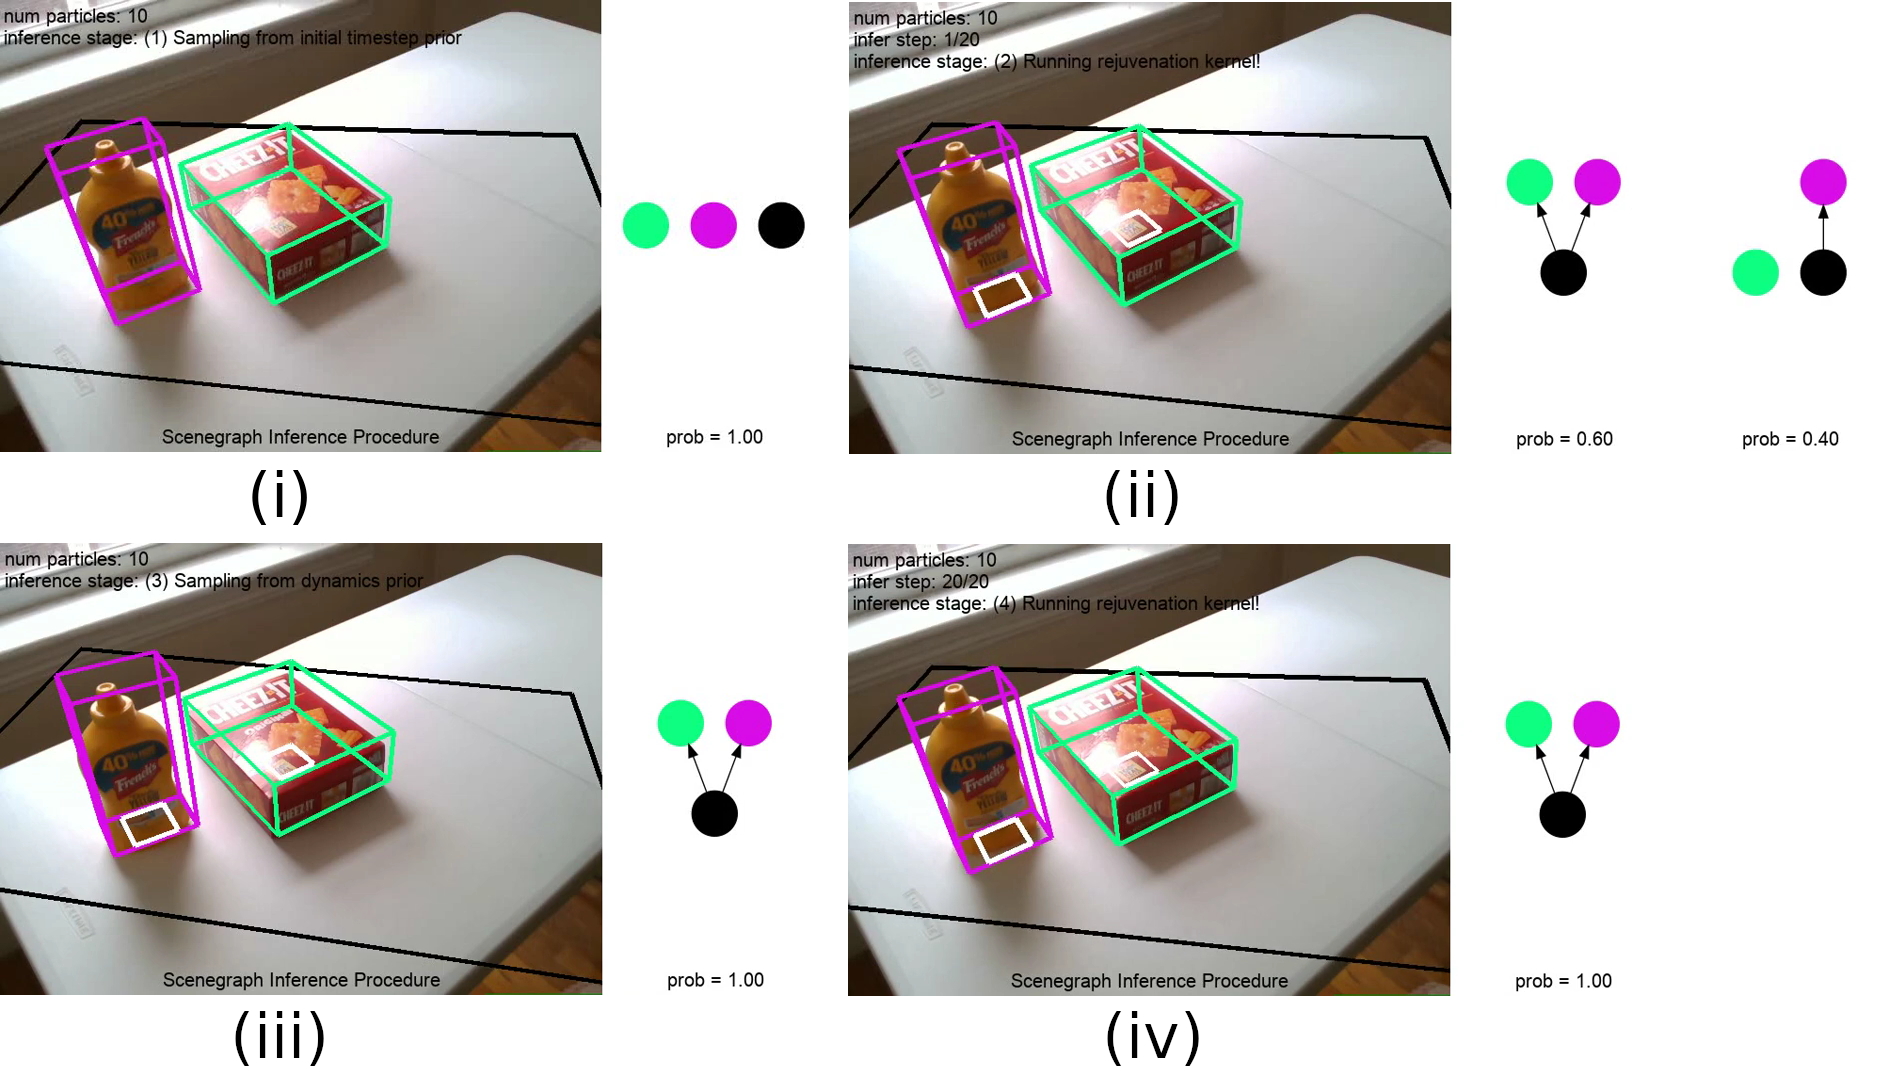
\includegraphics{particleFilterVis}
  \caption{
    Visualization of sampling and rejuvenation moves in a particle filter.
    A complete video of this scene can be seen at: \url{https://www.youtube.com/watch?v=0_0TvrGC65Q}.
    (i) shows the first time step with the overlaid beliefs from the initial time step prior (initialized to the observed neural pose estimates), before structure inference.
    (ii) shows the beliefs over the first time step, after running 1 step of the rejuvenation kernel.
    (iii) shows the beliefs over the second time step, after sampling from the dynamics model.
    (iv) shows the beliefs over the second time step, after running 20 steps of the rejuvenation kernel.
  }
  \label{fig:particleFilterVis}
\end{figure}

\subsection{Visualizing inference in a particle filter}
Finally, this section demonstrate a real-world application by showing the actual usage of these visualization utilities in a particle filter with a corresponding complex inference program.
This demonstrates how the methods introduced in this chapter can be used in practice for visualizing and debugging complex inference programs.
The scene graph model leverages the prior from~\ref{section:prior} and dynamics from~\ref{section:dynamics}.
Object poses are initialized to their observed neural detections in the first time step.
The inference program is based off of a rejuvenation MCMC kernel, after sampling from the prior for the first and second time step.
This kernel is in turn composed of an interleaved RJMCMC kernel (see~\ref{section:rjmcmc}) for discrete structure, and a drift kernel for continuous parameters.
The particle filter was ran with 10 particles, and 20 iterations of the rejuvenation kernel.
Figure~\ref{fig:particleFilterVis} uses the method in Figure~\ref{fig:multipleBeliefsBottom} to aggregate the particle filter state into a stable visual estimate of the mean object poses, and to view the distribution over inferred structure.
